\documentclass[10pt]{article}

\usepackage{amsmath}
\usepackage{graphicx}
\usepackage[margin=0.7in]{geometry}
\usepackage{float}
\usepackage{listings}
\usepackage[utf8]{inputenc}
\usepackage[parfill]{parskip}  
\usepackage{multicol}
\usepackage{siunitx}
\usepackage[dvipsnames]{xcolor}
% \usepackage{hyperref}
\usepackage{cleveref}
\usepackage{cite}
\usepackage{caption}
\usepackage{tabularx}
\usepackage{mathabx}
\usepackage{titling}
\usepackage{physics}

\captionsetup{width=0.6\linewidth}

\newcommand{\rhomax}{\rho_{\text{max}}}
\newcommand{\relerr}{\epsilon_{\text{rel}}}
\newcommand{\bigO}[1]{\mathcal{O}(#1)}

\graphicspath{{../results/}}

\newcommand\myshade{50}
\colorlet{mylinkcolor}{violet}
\colorlet{mycitecolor}{YellowOrange}
\colorlet{myurlcolor}{Aquamarine}

% \hypersetup{
%   linkcolor  = mylinkcolor!\myshade!black,
%   citecolor  = mycitecolor!\myshade!black,
%   urlcolor   = myurlcolor!\myshade!black,
%   colorlinks = true,
% }

% \pretitle{%
%     \begin{center}
%     \LARGE
%     }
% \posttitle{\end{center}}


\begin{document}
\title{The Ising Model
\\ Project 4
\\ FYS3150}
\author{Halvard Sutterud}
\date{November 2017}
\maketitle{\begin{center}\end{center}}
\pagenumbering{gobble}
\thispagestyle{empty}

\begin{figure}[H]
    \centering
    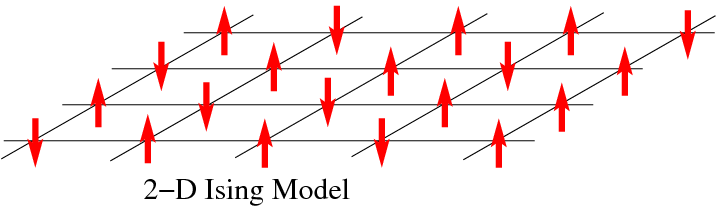
\includegraphics[width=0.8\linewidth]{../results/front.png}
    \caption{Temporary from http://inspirehep.net/record/1283384/files/ising.png}
    \label{fig:front}
\end{figure}

\begin{abstract}
    The Ising model in two dimensions is is used to simulate phase
    transitions in magnetic materials with a parallelized Metropolis
    algorithm. Critical temperature extracted, compared to
    \cite{PhysRev.65.117}.

    \begin{itemize}
        \item Give a short description of the nature of the problem and the eventual
        numerical methods you have used.
        \item Describe the algorithm you have used and/or developed. Here you may
        find it convenient to use pseudocoding. In many cases you can describe
        the algorithm in the program itself.
        \item Include the source code of your program. Comment your program properly.
        \item If possible, try to find analytic solutions, or known limits in order to test
        your program when developing the code.
        \item Include your results either in figure form or in a table. Remember to label
        your results. All tables and figures should have relevant captions and labels
        on the axes.
        \item Try to evaluate the reliabilty and numerical stability/precision of your
        results. If possible, include a qualitative and/or quantitative discussion of
        the numerical stability, eventual loss of precision etc.
        \item Try to give an interpretation of you results in your answers to the problems.
        \item Critique: if possible include your comments and reflections about the
        exercise, whether you felt you learnt something, ideas for improvements
        and other thoughts you’ve made when solving the exercise. We wish to
        keep this course at the interactive level and your comments can help us
        improve it.
        \item Try to establish a practice where you log your work at the computerlab.
        You may find such a logbook very handy at later stages in your work,
        especially when you don’t properly remember what a previous test version
        of your program did. Here you could also record the time spent on solving
        the exercise, various algorithms you may have tested or other topics which
        you feel worthy of mentioning.
    \end{itemize}
\end{abstract}

\newpage



\begin{multicols}{2}
\tableofcontents

% \newpage
\pagenumbering{arabic}

%%%%%%%%%%%%%%%%%%%%%%%%%%%%%%%%%%%%%%%%%%%%%%%%%%%%%%%%%%%%%%%%%%%%%%%%%%%
\section{Introduction}

%%%%%%%%%%%%%%%%%%%%%%%%%%%%%%%%%%%%%%%%%%%%%%%%%%%%%%%%%%%%%%%%%%%%%%%%%%%
\section{Theory}
The Ising Model is a binary system, where the objects at each lattice site
can take on two values, which we will take as spin up or spin down.

The energy of the Ising Model can generally be expressed as

\begin{equation}
    E = -J \sum_{<kl>}^N s_k s_l
\end{equation}

where $s_k = \pm 1$ is the orientation of the spin at a lattice point, and
the sum is to be taken only over the neighboring points.

\subsection{Units}
The energy is taken to be in units of $kT/J$.

\subsection{$2\times 2$ analytical calculation = 4a} 
\label{sub:2x2latticetheory}

\subsection{Studies of phase transition = pre 4e} 
\begin{itemize}
    \item Characterize behaviour of physical quantities as power law
        behaviour. 
    \item Correlation length $\xi$
    \item Second order phase transition $\Rightarrow$ $\xi \to L$.
\end{itemize}

%%%%%%%%%%%%%%%%%%%%%%%%%%%%%%%%%%%%%%%%%%%%%%%%%%%%%%%%%%%%%%%%%%%%%%%%%%%
\section{Methods}
\subsection{Main code, Metropolis algo = 4b}
We write a code for the Ising Model using the Metropolis algorithm and
periodic boundary conditions. MORE DETAILS HERE.

Given a size of the lattice grid $L$ in $x$ and $y$ directions, it
calculates the values of the mean energy $E$, mean magnetization $M$, the
specific heat $C_V$ and the susceptibility $\chi$ as functions of $T$ using
periodic boundary conditions.

\subsection{Equilibrium time = 4c}
The Metropolis algorithm is a stochastic method, we want to study how many
cycles are needed as a function of temperature. We do this by calculating
the various expectation values during a Metropolis run. 

\begin{itemize}
    \item Ordered and random state
    \item $T = 1$ and $T = 2.4$
\end{itemize}


\subsection{Parallelization = 4e (last part)}

%%%%%%%%%%%%%%%%%%%%%%%%%%%%%%%%%%%%%%%%%%%%%%%%%%%%%%%%%%%%%%%%%%%%%%%%%%%
\section{Results}
\subsection{Numerical vs 2x2 analytical = 4b}
\Cref{fig:2x2values} shows values in a simulation of a $2\times2$ lattice grid compared to
the analytical values from \cref{sub:2x2latticetheory}.

\begin{itemize}
    \item Number of MC cycles used
\end{itemize}

\begin{figure}[H]
    \centering
    \includegraphics[width=0.8\linewidth]{2x2values.pdf}
    \caption{2x2values}
    \label{fig:2x2values}
\end{figure}

\subsection{Reach most likely state = 4c}
Using a lattice size $L=20$, 

\begin{itemize}
    \item Number of MC cycles for equilibrium.\\
        $\Rightarrow$ equilibrium time ( MC cycles representing time )
    \item Total number of accepted configurations vs temperature
\end{itemize}


\subsection{Probability distribution = 4d}
After steady state situation is reached.

\begin{itemize}
    \item $P(E)$
    \item 
\end{itemize}


\subsection{Phase transition = 4e}
\label{sub:phase_transition}


behaviour as function of lattice size. $L \in {40, 60, 80, 100}$, $T \in
[2.0,2.3]$(or smaller?), $\Delta T < \SI{0.05}{K}$.

\begin{itemize}
    \item Plot $\ev E$,  $\ev{ |M| }$, $C_V$, $\chi$ vs $T$
\end{itemize}

\subsection{Method analysis = 4e (last part)}

\begin{itemize}
    \item timing analysis of gain from parallelization  
    \item optimal gain (whatever that is)
\end{itemize}

\subsection{Critical temperature = 4f}
Use $L \in {40, 60, 100, 140}$ to find the limit $L \to \infty$.

\begin{itemize}
    \item Compare with analytical from \cite{PhysRev.65.117}
\end{itemize}



%%%%%%%%%%%%%%%%%%%%%%%%%%%%%%%%%%%%%%%%%%%%%%%%%%%%%%%%%%%%%%%%%%%%%%%%%%%
\section{Discussion and conclusions}
\subsection{TENK PAA DENNE MENS DU GJOER RESTEN}
\label{sub:tenk_paa_denne_mens_du_gjoer_resten}




\section*{Appendix}
See https://github.com/halvarsu/FYS3150/projects/Project4 for code.

From \cite{lectureNotes}.

\bibliography{bib1}{}
\bibliographystyle{plain}

\end{multicols}


\end{document}
